\documentclass[10pt,a4paper,oneside]{article}
\usepackage[utf8]{inputenc}
\usepackage{amsmath}
\usepackage{amsfonts}
\usepackage{amssymb}
\usepackage{graphicx}
\usepackage{draftwatermark} % 设置水印
\SetWatermarkText{DNV Group} % 水印内容
\usepackage{breqn}
\usepackage{tikz} % system block diagram
\usepackage{textcomp}
\usetikzlibrary{datavisualization}
\usetikzlibrary{shapes,arrows} % system block diagram
\usepackage{booktabs}
\usepackage[framed,numbered,autolinebreaks,useliterate]{mcode} % matlab code block
\author{Yangang Cao}
\date{February 26, 2019}
\newcommand{\degree}{^\circ}
\tikzset{
	delay/.style    = {draw, thick, rectangle, minimum height = 3em,
		minimum width = 3em},
	sum/.style      = {draw, circle, node distance = 2cm}, 
	prod/.style     = {draw, circle, node distance = 2cm},
	input/.style    = {coordinate}, % Input
	output/.style  = {coordinate} % Output
}
% Defining string as labels of certain blocks.
\newcommand{\product}{$\displaystyle \times$}
\newcommand{\delay}{\large$z^{-1}$}
\begin{document}

\title{Compressor and Expander}
\maketitle 
While a limiter completely eliminates any dynamics above a certain threshold by keeping the output level constant, a compressor only reduces the dynamics, compressing the dynamic range. The reduced dynamics can be exploited to increase the overall level, thereby boosting the loud- ness, without exceeding the allowed amplitude range. An expander does just the opposite of the compressor, increasing dynamics by mapping small level changes of the input to larger changes of the output level. Applying an expander to low-level signals gives a lively sound characteristic. The corresponding ratios and slopes of the characteristic curve are $CR > 1$ and $0 < CS < 1$ for the compressor and $0 < ER < 1$ and $ES < 0$ for the expander.

Compressors and expanders typically employ RMS level detectors with an averaging time in the range $t = 5...130$ ms and a smoothing filter with $t_{AT} = 0.1...2600$ ms and $t_{RT} = 1...5000$ ms. 

Combining a compressor for high signal levels with an expander for low signal levels leads to
the gain computation
\begin{align*}
G &=
\begin{cases} 
CS\cdot(CT-X)   &\mbox{if } X>CT \\
0 \ \mbox{dB}  &\mbox{if }ET\leqslant X\leqslant CT\\
ES\cdot(ET-X) &\mbox{if }X<ET
\end{cases}\\
&=min(0, \ CS\cdot(CT-X),\ ES\cdot(ET-X)).
\end{align*}
Here CT and ET denote the thresholds above which the compressor and below which the expander affect the signal, respectively. The resulting combined system is depicted in following block diagram. 
\begin{center}
	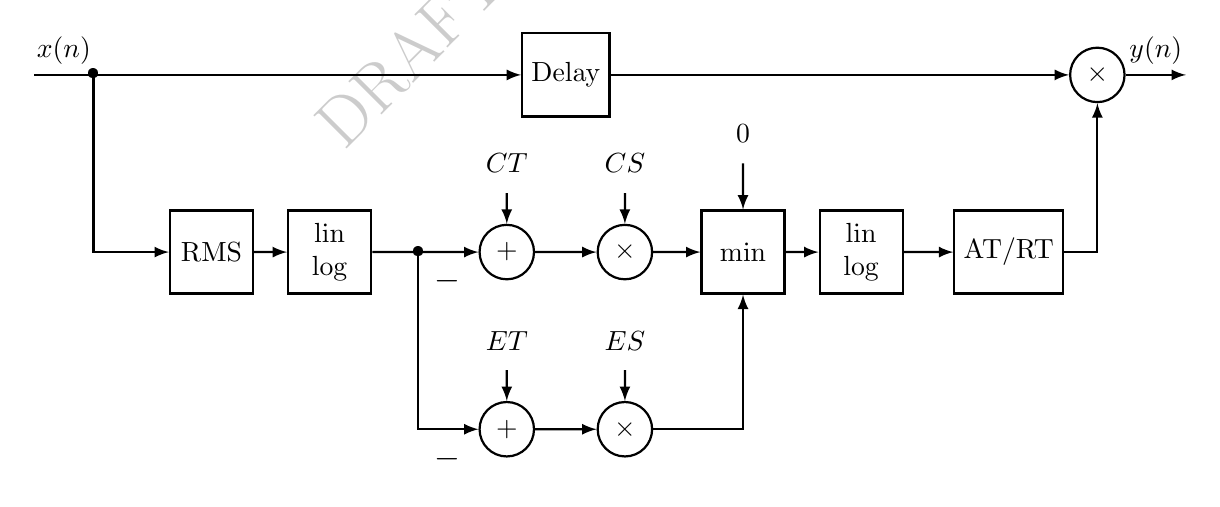
\begin{tikzpicture}[auto, thick, node distance=0.6cm, >=latex,scale = 0.75]
	\draw
	node at (5.5,-3) {\textbullet}
	node at (0,0)  {\textbullet}
	node at (2,-3) [delay] (d1) {RMS}
	node at (4,-3) [delay,align=center] (d2) {lin\\ log}
	node at (7,-3) [sum] (s1) {+}  node at (7,-1.5){$CT$}
	node at (9,-3) [prod] (p1) {\product} node at (9,-1.5){$CS$}
	node at (11,-3) [delay] (d3) {min}
	node at (13,-3) [delay,align=center] (d4) {lin\\ log}
	node at (15.5,-3) [delay] (d5) {AT/RT}
	node at (17,0) [prod] (p3) {\product}
	node at (8,0) [delay] (d6) {Delay}
	node at (7,-6) [sum] (s2) {+} node at (7,-4.5){$ET$}
	node at (9,-6) [prod] (p2) {\product} node at (9,-4.5){$ES$}
	node at (11,-1) {0}
	node at (6,-3.5) {\large$-$}
	node at (6,-6.5){\large$-$}
	;
	\draw[->](0,0)--(d6);
	\draw[->](d6)--(p3);
	\draw[->](0,0)|-(d1);
	\draw[->](d1)--(d2);
	\draw[->](d2)--(s1);
	\draw[->](s1)--(p1);
	\draw[->](p1)--(d3);
	\draw[->](d3)--(d4);
	\draw[->](d4)--(d5);
	\draw[->](d5)-|(p3);
	\draw[->](5.5,-3)|-(s2);
	\draw[->](s2)--(p2);
	\draw[->](p2)-|(d3);
	\draw[->](7,-2)--(s1);
	\draw[->](9,-2)--(p1);
	\draw[->](7,-5)--(s2);
	\draw[->](9,-5)--(p2);
	\draw[->](11,-1.5)--(d3);
	\draw[-](-1,0)--node {$x(n)$} (0,0);
	\draw[->](p3)--node {$y(n)$} (18.5,0);
	\end{tikzpicture}
\end{center}
 Again, the gain can alternatively be calculated without using logarithmic values by
\[
g ( n ) = \min \left( 1 , \left( \frac { x _ { \mathrm { RMS } } ( n ) } { c t ^ { 2 } } \right) ^ { - C S / 2 } , \left( \frac { x _ { \mathrm { RMS } } ( n ) } { e t ^ { 2 } } \right) ^ { - E S / 2 } \right),
\]
where the square root operation of the RMS measurement is moved to the exponenents by halving the respective slopes. This approach makes conversion to and from the logarithmic domain unnecessary, but requires exponentiation. An implementation following the approach is given in following {\bfseries Matlab} code.
\begin{lstlisting}
function y = compexp(audio, para)
% para(1): threshold of compressor (CT)
% para(2): slope factor of compressor (CS)
% para(3): threshold of expander (ET)
% para(4): slope factor of expander (ES)
tav = 0.01;
at = 0.03;
rt = 0.003;
delay = 150;
audiorms = 0;
g = 1;
buffer = zeros(1, delay);

for n = 1: length(audio)
	audiorms = (1 - tav) * audiorms + tav * audio(n)^2;
	X = 10 * log10(audiorms);
	G = min([0, para(2) * (para(1) - X), para(4) * (para(3) - X)]);
	f = 10^(G/20);
	if f < g
		coeff = at;
	else
		coeff = rt;
	end
	g = (1-coeff) * g + coeff * f;
	y(n) = g * buffer(end);
	buffer = [audio(n) buffer(1:end-1)];
end
\end{lstlisting}

A diagram of compression show in following figure, the output level changes softly when input level rises up to threshold abruptly, similar property occurs on expander. 
\begin{center}
	\includegraphics[height=150pt]{compression.eps} 
\end{center}
\end{document}
